\newpage
\section{Faraday Rotation}

\subsection{Execution}

\begin{figure}[!ht]
    \centering
    \includegraphics[width=0.85\textwidth]{img/setup3.png}
    \caption{Schematic of the setup used to record faraday rotation. As sample a WS$_2$ monolayer encapsulated within hBN layers on a \SI{500}{\micro\meter} thick c-cut sapphire substrate is used.}
    \label{fig_setup3}
\end{figure}
To measure the Faraday rotation of a WS$_2$ monolayer a novel setup by Dr. Ashish Arora and Dr. Benjamin Carey is used.
It is shown in \cref{fig_setup3} and allows a much faster acquisition of a whole spectrum than with previously used methods.
Here, two types of illumination are used:
Firstly, a laser to excite the monolayer and secondly a white light source to cover a broad energy spectrum rather than one energy at a time.
By using a laser line filter, the gaussian distribution of laser light energy is further monochromatized.
After polarizing the beam, it travels through the sample inside a magnetic field.
The transmitted light is then deflected into a lens system for reducing noise and focussing.
A key component in this setup is the beam displacer, where the beam splits into two relative to each other orthogonally polarized parts.
Their intensity difference is dependent on the Faraday rotation induced by the sample.
The beams are then both focused on different rows on the CCD-chip which is connected with a spectrometer.
Again, to remove the background light signal present in the laboratory, the signals of two additional rows around the ones where the beams are focused are taken and subtracted as background.
In the setup used for the acquisition, a read-out-rate of \SI{1}{\mega\hertz} is reached and allows measurement of roughly $1000$ spectra per minute.

\

According to the theoretical description in \cref{sec:theory}, measuring allows us to obtain the Faraday rotation, however with background.
As this background does not change with the polarization, measurements are taken at \SI{+45}{\degree} and \SI{-45}{\degree} (by introducing a $\lambda/2$-waveplate) and then subtracted, since the Faraday rotation changes sign.

To ensure that the WS$_2$ monolayer is laying flatly on a sapphire ($\text{Al}_2\text{O}_3$) substrate of \SI{500}{\micro\meter} thickness, it is trapped between hexagonal boron nitride layers, which only adds a negligible contribution to the measured data.
Since the beam passes through both, the sapphire substrate and the WS$_2$ monolayer, again two measurements have to be taken do differentiate the background from the monolayer.
This is done by comparing the Verdet constant of the monolayer with substrate to the Verdet constant of only substrate.

\subsection{Analysis}

\begin{figure}[!ht]
    \centering
    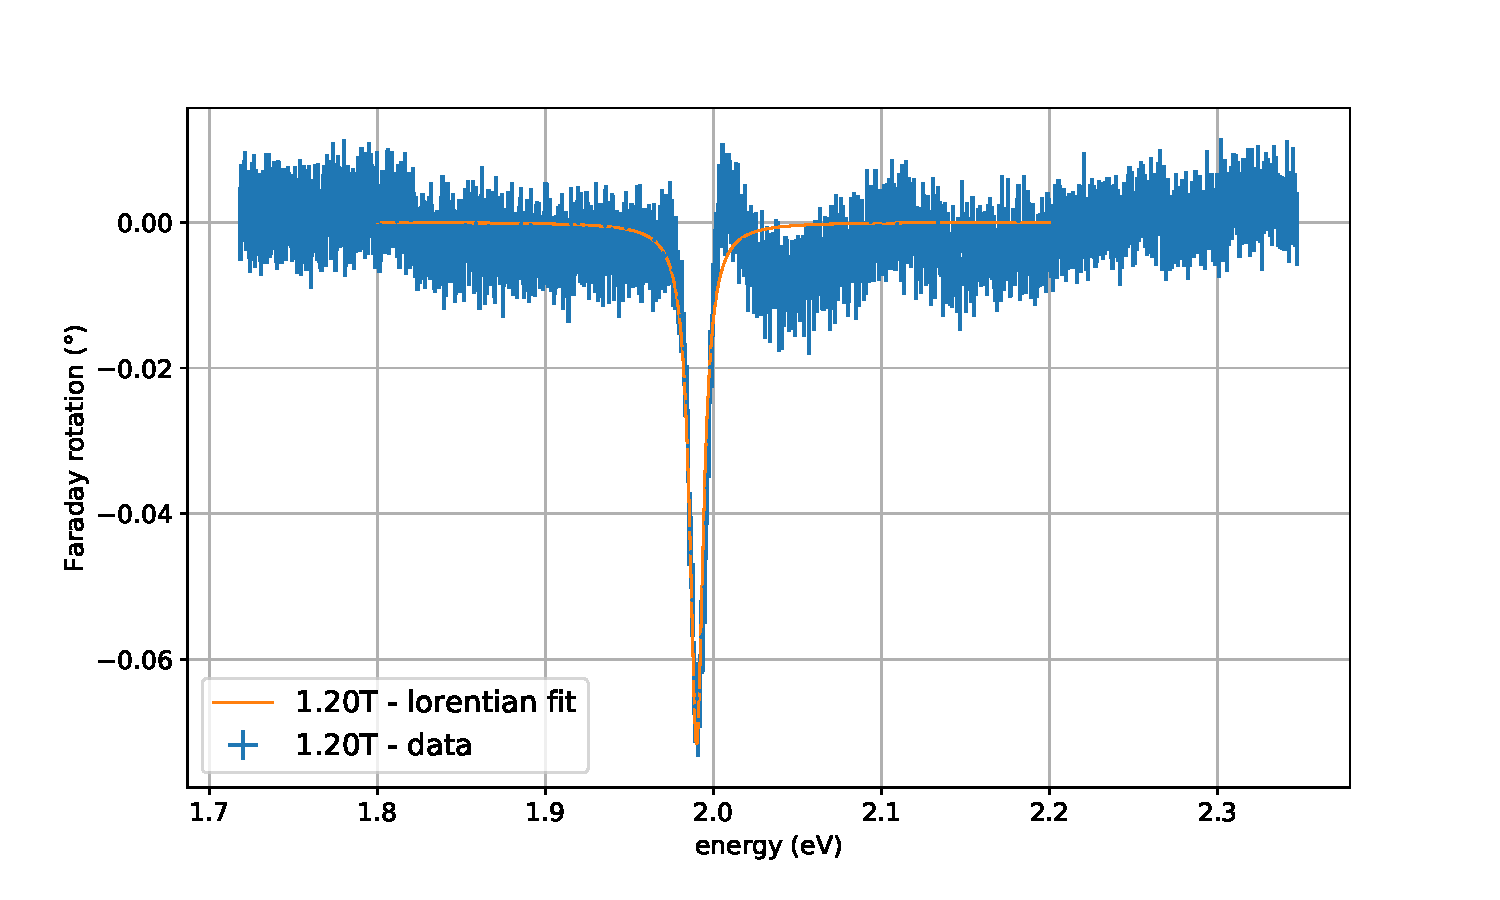
\includegraphics[width=0.85\textwidth]{plots/WS2_1200mT.pdf}
    \caption{Representation of WS$_2$ monolayer data points of the faraday rotation with external magnetic field of \SI{1.2}{\tesla} and lorentian fit.}
    \label{fig_WS2_1200mT}
\end{figure}
Since a lorentian line in the absorption spectrum is to be expected, lorentian fits are used to model the Faraday rotation spectrum of the WS$_2$ monolayer.
An example is given in \cref{fig_WS2_1200mT} at \SI{1.2}{\tesla}.
All other plots of the data and their corresponding lorentian fits can be found in the \cref{sec:anhang:far}.
For the uncertainties \SI{+-1}{\milli\tesla} for the external magnetic field and \SI{+-1}{\milli\electronvolt} for the energy are used.
The latter is due to the calibration error of the monochromator and the largest source of error.
Also in the \cref{sec:anhang:far} is a plot without errorbars, namely \cref{fig_WS2_250mT_noerror}.
From the scattering of data points outside of the exciton region, an uncertainty of \SI{+-0.005}{\degree} is extracted and used for the faraday rotation in other plots and calculations.

\begin{figure}[!ht]
    \centering
    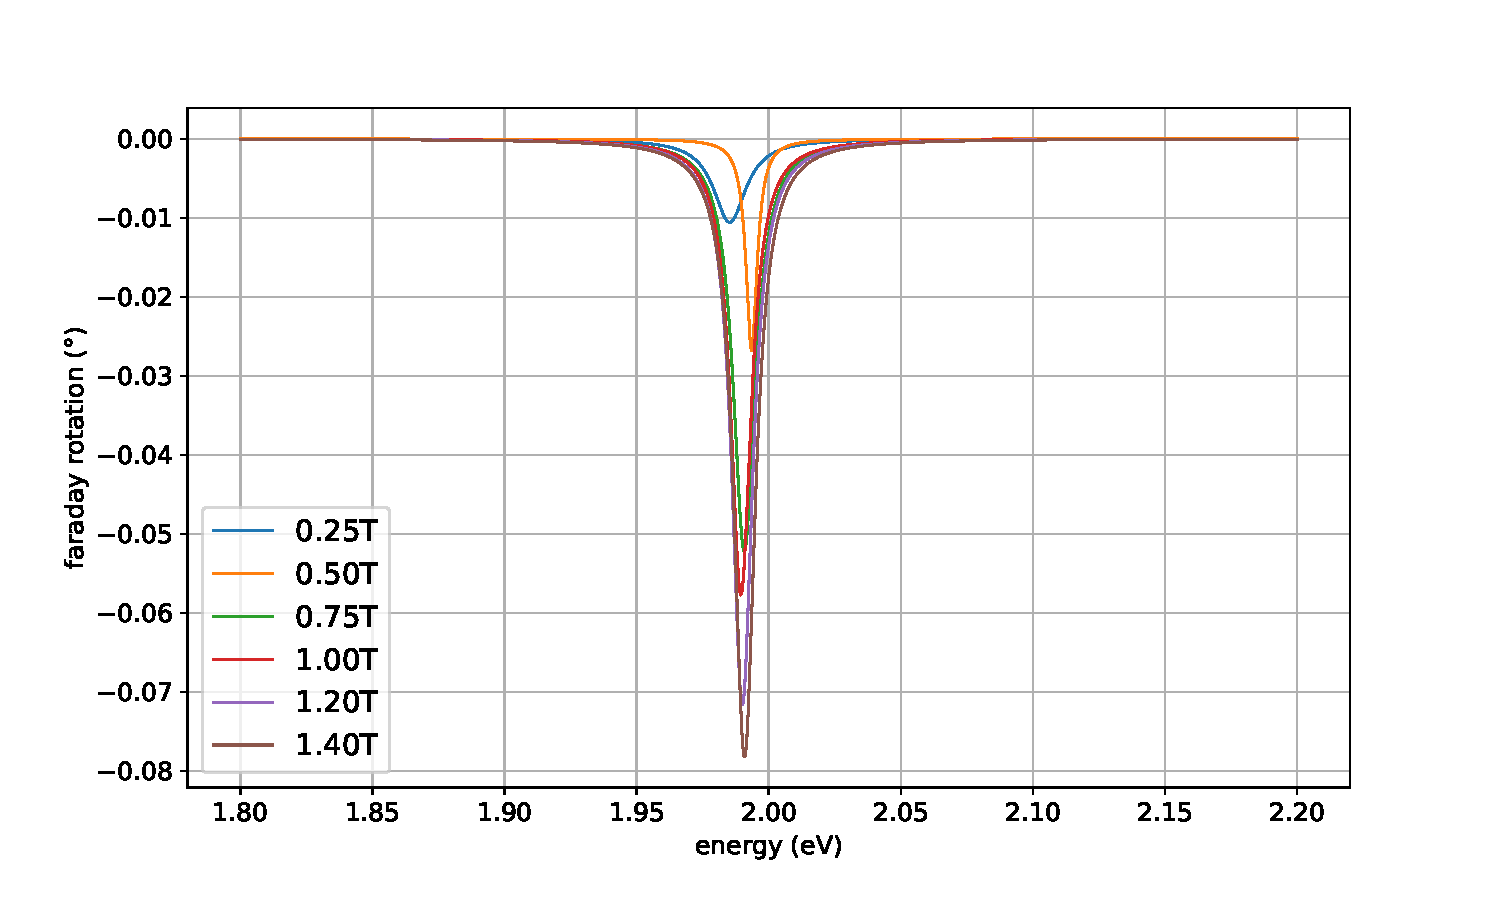
\includegraphics[width=0.85\textwidth]{plots/WS2_lorentians.pdf}
    \caption{Representation of all lorentian fits plotted together.}
    \label{fig_WS2_lorentians}
\end{figure}
For comparison all lorentian fits are found in \cref{fig_WS2_lorentians}.
The Faraday rotation at the exciton energy rises almost linearly as a function og the magnetic field.
Only the minimum at \SI{0.75}{\tesla} does not fit very well.
This may be due to imperfection in choosing the same sample position, or a small movement of the sample spot during the measurement time.
Also, the energy of the minima is not exactly the same for all magnetic field strengths, as it should be.
However, since they are almost the same, the mean value of \SI{1.990+-0.001}{\electronvolt} gives a good estimate.

\begin{figure}[!ht]
    \centering
    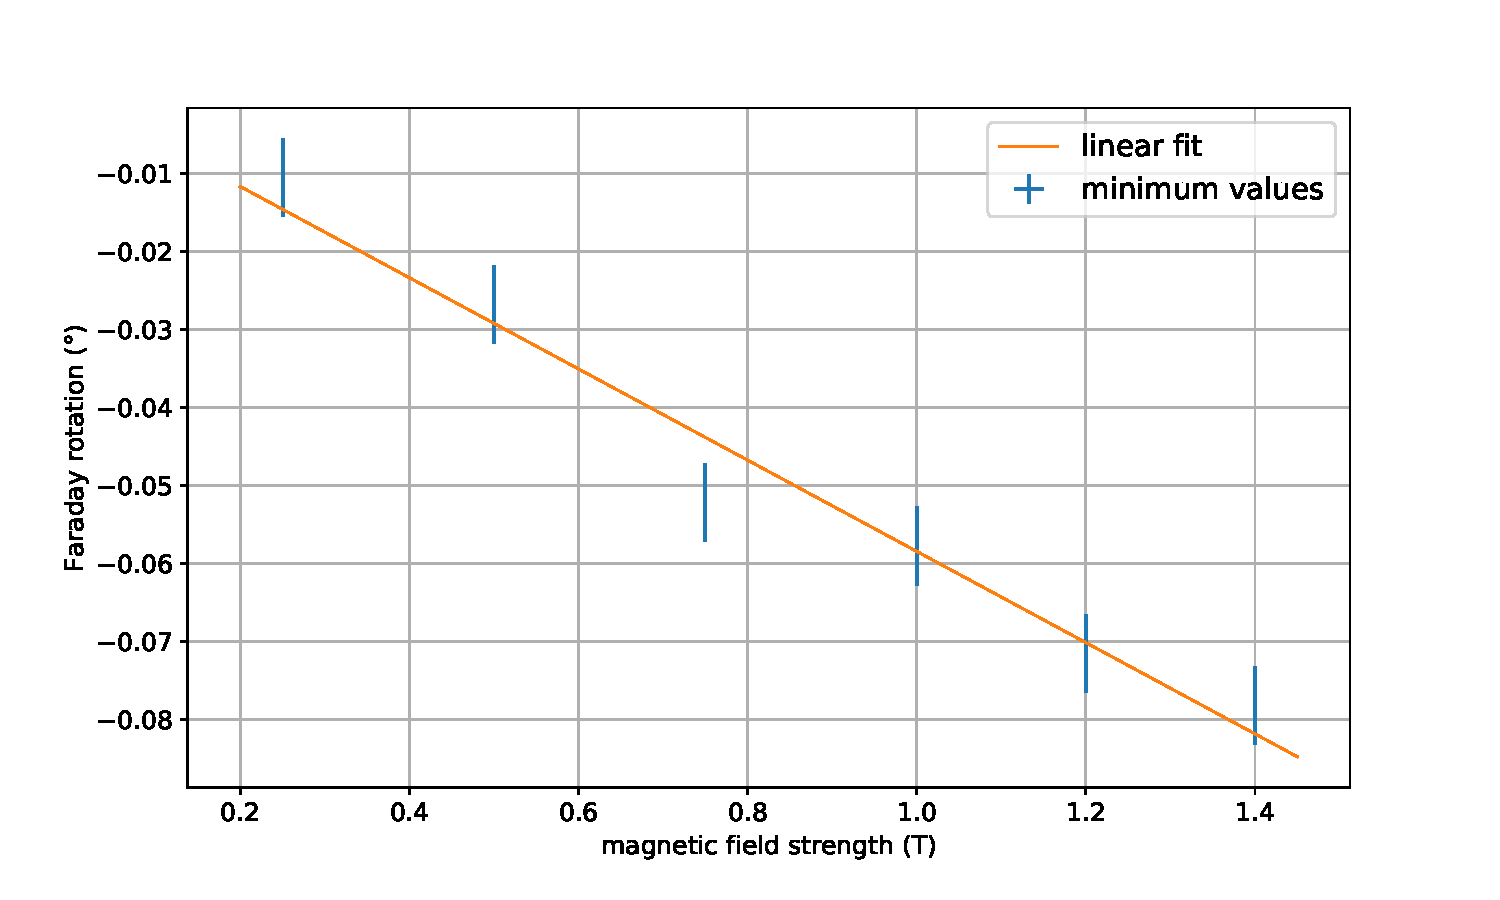
\includegraphics[width=0.85\textwidth]{plots/WS2_mins.pdf}
    \caption{Representation of largest WS$_2$s faraday rotation in dependence of external magnetic field strength.}
    \label{fig_WS2_minima}
\end{figure}
Figure \ref{fig_WS2_minima} shows the beforementioned linear decrease by plotting the minima against the magnetic field strength.

From its slope the Verdet constant is extracted by division of the monolayers thickness of \SI{0.65}{\nano\meter}.
It amounts to \SI{-8.99+-0.31e+07}{\deg m^{-1} T^{-1}}.

\

\begin{figure}[!ht]
    \centering
    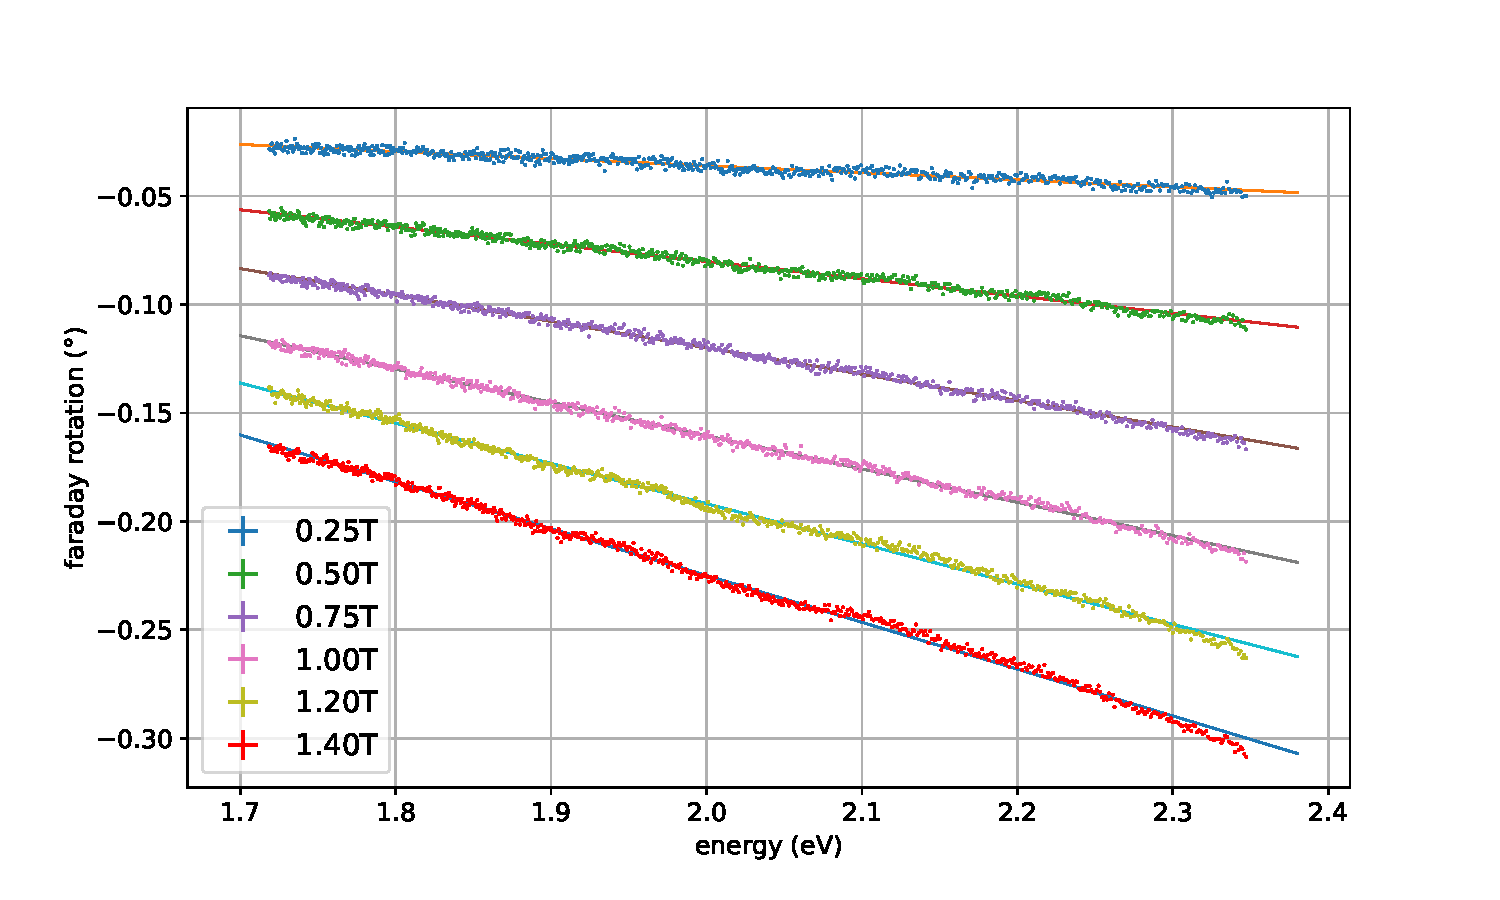
\includegraphics[width=0.85\textwidth]{plots/sapphire_lins.pdf}
    \caption{Representation of sapphire data points of the faraday rotation with different external magnetic fields and linear fits.}
    \label{fig_sapphire_lins}
\end{figure}
Contrary to the exciton contribution, only a linear increase in the magnitude of the Faraday rotation with rising energy is seen for the sapphire substrate in \cref{fig_sapphire_slopes}.
The data at each energy is fitted linearly over all magnetic field strengths, as in \cref{fig_WS2_minima}.
By dividing these values by the sapphire's thickness of \SI{500}{\micro\meter} and plotting them in \cref{fig_sapphire_verdet}, the energy dependent Verdet constant for sapphire is visualized.

\begin{figure}[!ht]
    \centering
    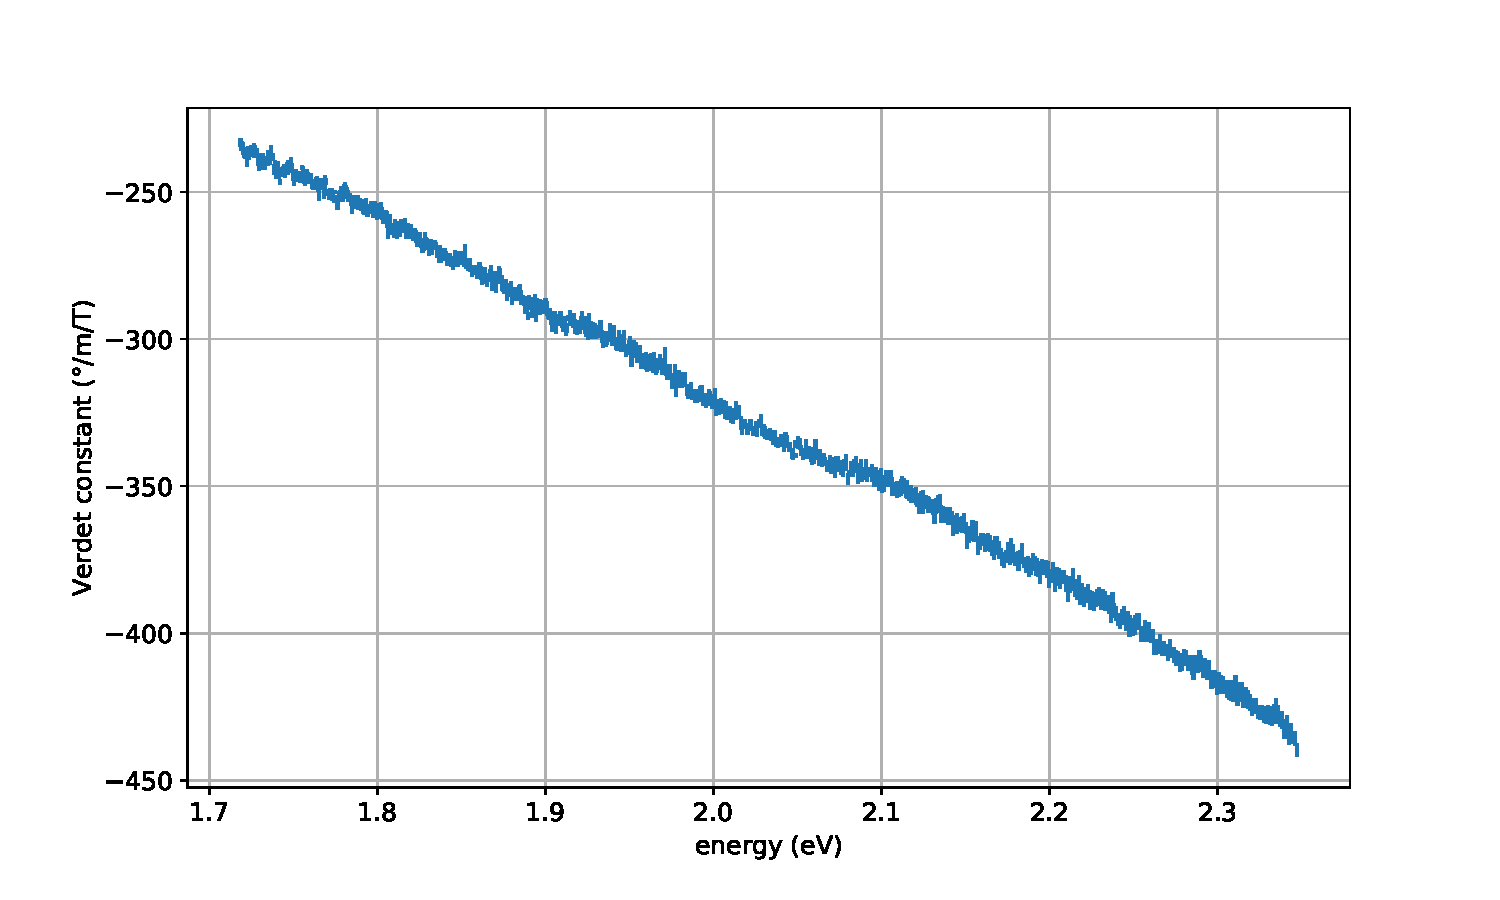
\includegraphics[width=0.85\textwidth]{plots/sapphire_verdets.pdf}
    \caption{Representation of sapphire's Verdet constant in dependence of energy.}
    \label{fig_sapphire_verdets}
\end{figure}

These values are all of an order of \SI{e+02}{{\deg m^{-1} T^{-1}}} and therefore differ by five orders of magnitude from the \SI{-8.99+-0.31e+07}{\deg m^{-1} T^{-1}} of the WS$_2$ monolayer at the exciton energy.
This shows how strongly excitons influence the faraday rotation.
